%% Template for a preprint Letter or Article for submission
%% to the journal Nature.
%% Written by Peter Czoschke, 26 February 2004
%%

\documentclass{natureJMK}

\usepackage{graphicx}
\usepackage{bkdefs}
\usepackage[plain]{fancyref}
\renewcommand*{\Freffigname}{Fig.}
\renewcommand*{\freffigname}{Fig.}

%% make sure you have the nature.cls and naturemag.bst files where
%% LaTeX can find them
\newcommand{\tempS}[1]{}

\bibliographystyle{naturemag}

\title{Submesoscale streamers exchange water on the North Wall of the Gulf Stream}

%% Notice placement of commas and superscripts and use of &
%% in the author list

\author{Jody M. Klymak$^{1}$, R. Kipp Shearman$^2$, Jonathan Gula$^3$, Craig M. Lee$^4$, Eric A. D'Asaro$^4$, Leif N. Thomas$^5$, Ramsey Harcourt$^4$, Andrey Shcherbina$^4$, Miles A. Sundermeyer$^6$, Jeroen Molemaker$^3$ \& James C. McWilliams$^3$}

\begin{document}

\maketitle

\begin{affiliations}
 \item University of Victoria, Victoria, British Columbia, Canada
 \item Oregon State University, Corvallis, Oregon, USA
 \item University of California, Los Angeles, California, USA 
 \item Applied Physics Laboratory, University of Washington, Seattle, Washington USA
 \item Stanford University, Stanford, California, USA
 \item University of Massachusetts Dartmouth, Dartmouth, Massachusetts, USA
\end{affiliations}

\begin{abstract}
The Gulf Stream is a major conduit of warm surface water from the tropics to the subpolar North Atlantic.  Its north side has a strong  temperature and salinity front that is maintained for hundreds of kilometers, despite considerable energy available for mixing.  Large mesoscale ($\mathbf{>20}$ km) ``rings'' often pinch off, but like the Gulf Stream they are resistant to lateral mixing, and retain their properties for a long time.  Here we observe and simulate a sub-mesoscale ($\mathbf{<20}$ km) mechanism by which the Gulf Stream exchanges water with the cold subpolar water to the north: a series of ``streamers'' that detrain partially mixed water from the Gulf Stream at the crest of meanders. Subpolar water is entrained that replaces the partially mixed water, helping to resharpen the front. The water mass exchanges can account for lateral diffusivities if 125-250 $\mathbf{m^2\,s^{-1}}$, enough to supply the fresh water required for the production of 18-degree subtropical mode water.  
\end{abstract}

The Gulf Stream is the western boundary current of the North Atlantic subtropical wind-driven circulation.  It separates from Cape Hatteras and extends into the interior North Atlantic traveling east.  As it does so, it loses heat not only to  the atmosphere, but also the to waters in the subpolar gyre to the north.  The Gulf Stream entrains water from both the north and south, increasing its eastward transport by approximately 4-8 Sv/100 km \cite{johnsetal95}.    It cools, primarily from atmospheric forcing, but also due to significant lateral exchanges \cite{joyceetal13}.  

The Gulf Stream has a strong density front, but even along isopycnals there is a  sharp temperature-salinity front along the north wall of the Gulf Stream.  Salinity decreases by almost 1.5 psu moving north across the front, compensated in density by a drop in temperature of almost $5\mathrm{^oC}$.   The sharpness of this front persists for 100s of kilometers.  The front happens along constant density surfaces, which usually are not a barrier to mixing. However, the Gulf Stream water has a very high potential vorticity gradient (angular momentum; see methods) that is believed to act as a barrier to mixing on large scales \cite{marshalletal06,naveiraetal11}.  

Despite this  barrier and the presence of the sharp stable front, budgets of properties of the Gulf Stream indicate that there is significant exchange across the North Wall\cite{joyceetal13}.  Fresh water is entrained, and is necessary to create the dynamically important ``18 degree water'' that fills much of the upper Sargasso Sea. There are large eddies that periodically pinch off and carry warm water to the north. However, some of these are re-entrained into the Gulf Stream, and tracer budgets across the front appear to be dominated by small-scale processes\cite{boweretal85}. To date some of the best direct evidence for cross-front exchange consists of the trajectories isopycnal (constant density) floats placed on the North Wall \cite{bowerrossby89,bowerlozier94}.  These floats were observed to regularly detrain from the Gulf Stream, such that of 95 floats, 26 stayed in the Gulf Stream, 7 were detrained in rings, and 62 were detrained by mechanisms other than rings\cite{bowerlozier94}.  Some floats that detrained were also observed to move upwards rapidly in motions that were clearly ageostrophic.  
%TODO: Make these paras shorter

Here we present evidence of small scale lateral mixing ($<$0.5 km)  of the Gulf Stream (GS) on its northern cyclonic side, and that this partially mixed water periodically peels off the Gulf Stream in thin (5-10 km wide) ``streamers''.  The streamers carry  warm, salty, and high-vorticity  water north of the stream.  Because they have cyclonic vorticity anomaly, they also wrap up cold fresh water and entrain it into the GS.  The preferential detrainment of partially mixed water explains the persistent sharpness of the GS front despite the presence of mixing processes at the base of the GS.  We also speculate that the preferential detrainment of this water into the streamers is dynamically linked to the partial mixing of vorticity at the base of the GS. 

In March 2012 we made high-resolution measurements of the North Wall of the GS from 66 W to 60 W (\fref{fig:SatOverviewSectD}), about 850 km east of where the stream separates from the North American continental slope.  Two research vessels followed a Lagrangian float placed in the GS front at $\sigma_{\theta}=XX\ \mathrm{kg\,m^{-3}}$.  The float was advected downstream with an average (and relatively constant) speed of 1.4 $\mathrm{m\,s^{-1}}$. It progressively moved to denser water as the surface of the GS cooled downstream.  One vessel maintained  tight sampling around the float and deployed an undulating profiler to 200 m, making 10-km cross sections every 10 km downstream.  The second vessel  had an undulating profiler making larger 30-km  scale sections.  Both profilers measured temperature, salinity and pressure, and had approximately 1-km along-track resolution; both ships also measured ocean currents.  By following the float, a focus on the front was maintained as it curved and meandered to the east.  

The GS had a shallow meander crest (65 W, \fref{fig:SatOverviewSectD}b)  followed by a long concave region (63 W) and then another large  crest (61 W).  Satellite measurements show the sharp temperature changes across the front, superimposed with thin intermediate-temperature (15-18$^o$C) streamers detraining to the north at approximately 65 W, 64 W, and at the crest of the large meander at 61 W.  An older streamer that has rolled up can also be seen at 62 W.  The ships passed through the three newer streamers giving observations of these streamer's underwater structure.  

The front consists of density surfaces that slope up towards the north (\fref{fig:SalDFirstStreamer}a-d).  Salinity (coloured) along the density surfaces is salty (and warm) in the Gulf Stream, and fresher (and cold) to the north.  The lateral contrast between the two waters is amongst the largest and sharpest in the ocean, with salinity changing almost 1 psu over 5 km.  The temperature-salinity relationship shows the contrast between the two water masses as two distinct modes (\fref{fig:ComposeTSfigNew}a).  There is also a third less-populated but distinct population between the two larger modes in T/S space that we term the ``streamers''.  These manifest themselves in the cross-sections as intermediate salinity anomalies ($S \approx 36.15\ \mathrm{psu}$; \fref{fig:SalDFirstStreamer}a--d).  Along $\sigma_{\theta}=26.25\ \mathrm{kg\,m^{-3}}$, these anomalies are horizontally connected (\fref{fig:ComposeTSfigNew}b), peel off the north wall of the GS, are 5-10 km wide, and are stretched out for almost 50 km along the wall. The streamers have a strong potential vorticity signature (equivalent to angular momentum; see Methods).  Along the $\sigma_{\theta} = 26.25$ isopycnal, the region of high potential vorticity corresponds in space very well with the partially mixed ``streamer'' water (\fref{fig:SalDFirstStreamer}i--l, \fref{fig:ComposeTSfigNew}b ).   

The streamers remove water from the Gulf Stream frontal region.  The velocity contrast across the front is  sharp, with $>1\ \mathrm{m\,s^{-1}}$ drop in 5 km (\fref{fig:SalDFirstStreamer}e--h, \fref{fig:ComposeTSfigNew}b ).  The streamers start on the fast side of the front, moving approximately $0.25\ \mathrm{m\,s^{-1}}$ faster than the float (\fref{fig:SalDFirstStreamer}h). Upstream, where they are detached (\fref{fig:SalDFirstStreamer}e) they are moving almost $0.5\ \mathrm{m\,s^{-1}}$ slower.  This represents a considerable detrainment from the Gulf Stream.  If we assume a 5-km wide and 150-m deep streamer detraining at a relative velocity of $0.75\ \mathrm{m\,s^{-1}}$, then each streamer represents a loss of over $0.5\times10^{6}\, \mathrm{m^{3}\,s^{-1}}$ of water.  

The streamers move up through the water column along isopycnals and the water parcels are stretched vertically. The streamer in \fref{fig:ComposeTSfigNew}a has risen along isopycnals from 140 m deep (\fref{fig:ComposeTSfigNew}d)  to less than 40 m deep, and titled somewhat as it has done so.   The velocity anomaly is about $0.75\ \mathrm{m\,s^{-1}}$ over 100 km so we estimate that the streamer is approximately 1.5 days old,  implying vertical velocities on the order of 50 m/day, similar to rates inferred from large-scale omega-equation calculations\cite{thomasjoyce10}.  

High-resolution numerical simulations ($dx\approx 500 m$, see Methods) are able to resolve these features and tell a similar story (\fref{fig:StreamersModel}). Seeding the simulation with tracked particles (see methods) allows us to track the evolution of the streamers as the flow moves downstream.  Before the streamer is formed, the fresh water (blue contours) is near the surface and the salty water (green contours) is well within the front (\fref{fig:StreamersModel}a,b).  Downstream (\fref{fig:StreamersModel}c,d) the fresh water has been subducted dramatically to 150 m depth, and the salty streamer has been pushed north of the front.  Both water masses accelerate with the whole GS between these two snapshots (\fref{fig:StreamersModel}e), but the fresh water accelerates more, such that the fresh water is entrained and the salty water slows and is detrained.  As in the data, the streamer water occupies an intermediate region in T-S space (\fref{fig:StreamersModel}f, green contour).  

The acceleration of the fresh water relative to the salty is an important finding of the model, as the fresh water now represents a new sharp T-S front with the warm salty GS, and the partially mixed streamer water is carried away from the front.  The model also shows that the streamers are more prominent on the leading edges of meanders.  There are differences with the data, however.  The data shows very distinct T-S signatures associated with the streamers, whereas in the model the streamer T/S ``mode'' is less isolated (\fref{fig:StreamersModel}f).  The two interleaving water masses are also very isopycnal in the model, with the fresh water being slightly lighter than the salty, whereas in the data both water masses  share and cut across isopycnals (compare \fref{fig:SalDFirstStreamer}b to \fref{fig:StreamersModel}d).   There is also clear evidence of strong subduction of the cold water in the model, reminiscent of intrathermocline eddies \cite{thomasjoyce10} but is dissimilar to the cross-isopycnal interleaving shown in the data above.    

Differences between the data and the model aside, there are two major implications to this loss of partially mixed water to the north.  The first is that it helps explain why the front at the north wall of the Gulf Stream remains so sharp.  It is not that there is no mixing taking place in both the horizontal and the vertical, but rather that the mixing product is carried away in the ``streamers''.  It is striking that it is only partially mixed water that is carried away, and not high-salinity GS water (\fref{fig:ComposeTSfigNew}m), and that this is also high-vorticity water.  This implies a dynamical link that we have not seen explored.  Streamers have been observed from surface temperature in satellites and floats \cite{bowerrossby89,flierletal87,lozieretal97 ,songetal95}, and this has led to kinematic models in which particles are displaced from streamlines going around propagating meanders \cite{bower91,prattetal95,lozieretal97}. The observations here add to these models that it is only partially mixed water leaves the Gulf Stream.  This co-incidence indicates to us a role for small-scale mixing in producing the partially mixed water and the destabilizing forces that cause this water to detrain from the north wall.  The observations and simulation indicate that the meanders of the GS play an important role.  

The second implication is that the detrainment works against a salinity gradient and therefore we can calculate a lateral diffusivity.  If there is a meander every 200 km, and each meander detrains 0.5 Sv of fluid over 200 m depth, then a rough northward velocity associated with the turbulent structure is $v'=0.0125\ \mathrm{m\,s^{-1}}$.  Acting over a north-south length scale of $Y'\approx 10-20 \mathrm{km}$, we get a lateral diffusivity of $K_H=125-250\ \mathrm{m^2\,s^{-1}}$.  This is similar to diffusivities from inverse calculations using oxygen, temperature, and salinity\cite{boweretal85,joyceetal13}. The observations directly observe this diffusivity, rather than inferring it from inverse calculations. This inferred large-scale diffusivity is the right size and needed to bring fresh water into the Gulf Stream in order for 18 degree water to be formed further downstream.\cite{joyceetal13}

Here we have observed a  lateral mixing process on the North Wall of the Gulf Stream.  The streamers lose warm salty water to the north and bring cold fresh water into contact with the North Wall, hence resharpening the lateral gradients.  Closer inspection reveals interleaving of high- and low-salinity water along the entire North Wall, indicating a smaller scale lateral mixing process maybe important (see the alternating green and yellow in \fref{fig:ComposeTSfigNew}n).  There is also thought to be significant mixing due to other process such as symmetric instability \cite{thomasetal15}, inertial waves\cite{whittthomas13}, perhaps enhanced by cabelling.  


\section{Methods}

The Lagrangian float was placed in the Gulf Stream front based on a brief cross-stream survey with a target isopycnal of ??ERIC??.  The float moved downstream at a mean speed of 1.4 $\mathrm{m\,s^{-1}}$.  The \emph{R/V Knorr} tracked the float and deployed a Chelsea Instruments TriAxus that  collected temperature, salinity, and density (CTD) on a 200-m deep sawtooth with approximately 1-km horizontal spacing over short 10-km long sections that were approximately boxes in the float's frame (\fref{fig:SatOverviewSectD}, magenta).  \emph{R/V Atlantis} maintained a larger set of cross sections approximately 30 km across the front, trying to intercept the float on each front crossing.  \emph{R/V Atlantis} was deploying a Rolls Royce Marine Moving Vessel Profiler equipped with a CTD that profiled to 200 m approximately every 1 km.  Both ships had a 300 kHz RDI Acoustic Doppler Current Profiler (ADCP) collecting currents on 2-m vertical scale averaged every 5 minutes (approximately 1 km lateral scale), collected and processed using UHDAS and CODAS (http://currents.soest.hawaii.edu\cite{firingetal12}).  This data reached about 130 m, and was supplemented at deeper depths with data from 75 kHz RDI ADCPs, with 8-m vertical resolution.  

Data were interpolated onto density surfaces by creating a two-dimensional interpolation onto a grid at each depth via linear interpolation of a Delauney triangulation. No extrapolation was performed.  Data on the $26.25\ \mathrm{kg\,m^{-3}}$ isopycnal were assembled at each grid point by finding the first occurrence of that isopycnal in depth.  

Potential vorticity is calculated from the three-dimensional grid as the product of velocity curl ($\nabla\times\mathbf{u}$) added to the Coriolis vector ($\mathbf{f}$) and buoyancy gradients ($\frac{g}{\rho_0}\nabla\rho$):
\begin{equation}
  q = \frac{g}{\rho_0}\left(\nabla\times\mathbf{u}+\mathbf{f}\right) \cdot \nabla\rho,
\end{equation}
there the bracketed term is twice the angular velocity, including the planet's rotation, and the gradient of density represents the stretching or compression of the water column.  In the Gulf Stream, the potential vorticity is dominated by contributions from the vertical terms, and the cross-stream gradient of the along-stream velocity:
\begin{equation}
  q \approx N^2\left(-\frac{\partial u}{\partial y}+f\right).
\end{equation}

Numerical simulation. The high-resolution realistic simulation of the Gulf Stream is performed with the Regional Oceanic Modeling System (ROMS\cite{shchepetkinmcwilliams05}). This simulation has a horizontal resolution of 500m and 50 vertical levels. The model domain spans 1,000 km by 800 km and covers a region of the Gulf Stream downstream from its separation from the U.S. continental slope. Boundary conditions are supplied by a sequence of two lower-resolution simulations that span the entire Gulf Stream region and the Atlantic basin, respectively. The simulation is forced by daily winds and diurnally modulated surface fluxes. The modelling approach is described in detail in Gula et.\ al\cite{gulaetal15}.

Virtual Lagrangian Particles.  The neutrally buoyant Lagrangian (flow-following) particles were seeded at time 285 and advected both backwards and forwards from this time by the model velocity fields without any additional dispersion from the model's mixing processes\cite{gulaetal14}. A 4th-order Runge-Kutta method with a small time step size $dt = 1\ \mathrm{s}$ is used to compute particle advection. Velocity and tracer fields are interpolated at the positions of the particles using cubic spline interpolation in both the horizontal and vertical directions.  We use hourly outputs from the simulation to get sufficiently frequent and temporally-smooth velocity sampling for accurate parcel advection.



\begin{figure*}[htbp]
  \centering
    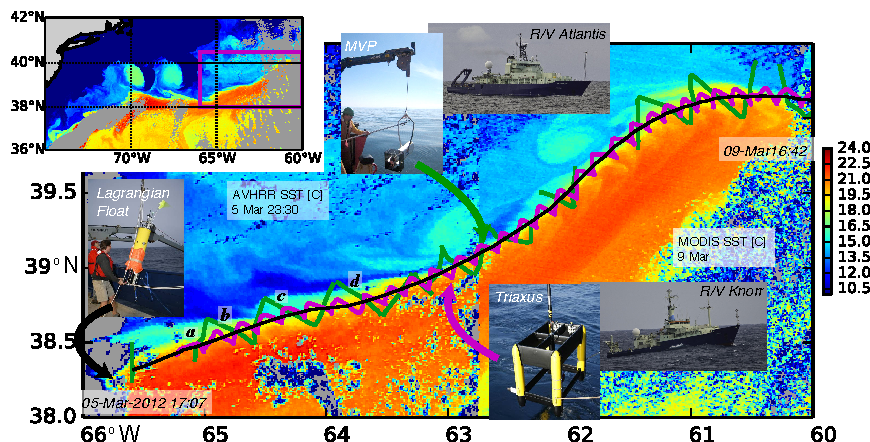
\includegraphics[width=\textwidth]{./SatOverviewSecDTry2.pdf}
   \caption{{\bf Experimental design.}  Inset: The experiment site on the north wall of the Gulf Stream, between 66 and 60 W, as shown in an AVHRR satellite image of sea surface temperature (SST).  Main:  Detailed SST image composed from two satellites images.    The Gulf Stream is warm and delineated by a sharp front.  There are small sub-mesoscale structures north of the front, which are the focus of this paper.  The satellite images are a composite from early in the observation period (AVHRR 6 Mar), and late (MODIS, 9 Mar).  A Lagrangian float was deployed in the front (black curve), and the ship tracks bracketed the float's position (green: \emph{R/V Atlantis}, magenta: \emph{R/V Knorr}).   }\label{fig:SatOverviewSectD}
\end{figure*}

\begin{figure*}[htbp]
  \centering
    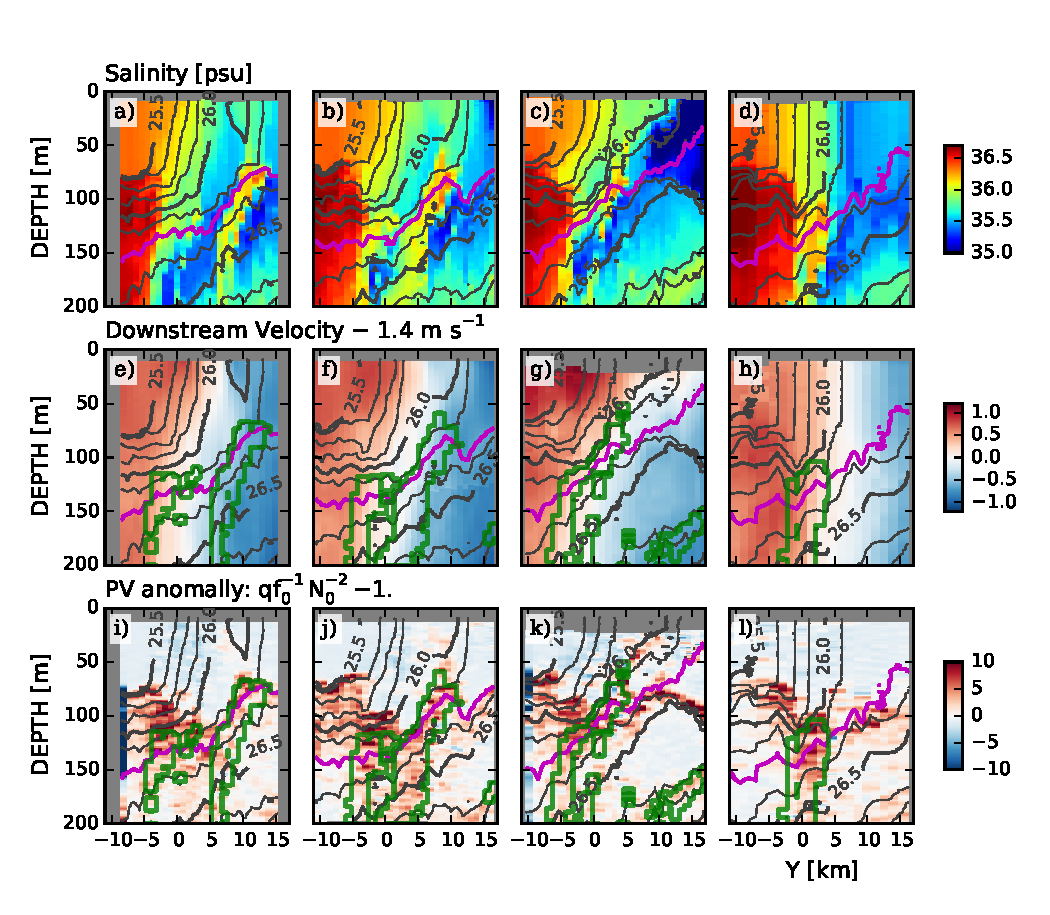
\includegraphics[width=\textwidth]{./SalDFirstStreamer.pdf}
    \caption{{\bf Cross sections of data collected across the Gulf Stream.}   $Y$ is the cross-stream distance perpendicular to the path of the float, positive being northwards (\fref{fig:SatOverviewSectD}). Potential density is contoured in black and $\sigma_{\theta}=26.25\ \mathrm{kg\,m^{-3}}$ is magenta.  Along a constant density surface salty water is warmer than fresher water, so the Gulf Stream on the left is warm and salty.  a) is the furthest upstream section (65W) and d) is the furthest downstream (63.75 W) (\fref{fig:ComposeTSfigNew}b).  e)--h) downstream velocity calculated relative to the float's trajectory by removing the float's mean speed of $u_{float}=1.4\ \mathrm{m\,s^{-1}}$ for the observation period.   Green contours are regions in temperature-salinity space labeled ``streamers'' in \fref{fig:ComposeTSfigNew}a.  i)--l) Potential vorticity sections (angular momentum - see text); 
 } \label{fig:SalDFirstStreamer}
\end{figure*}


\begin{figure*}[htbp]
  \centering
    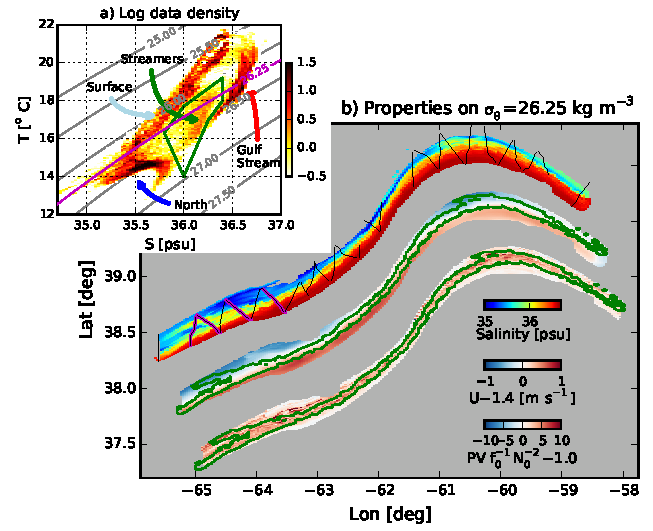
\includegraphics[width=0.9\textwidth]{./ComposeTSfigNew.pdf}
  \caption{{\bf Streamer properties and distribution in space.}
a) Logarithmically scaled histogram
 in temperature-salinity space (colours). The warm-salty Gulf Stream water is very distinct from the water to the north, which is cold and fresh.  The water near the surface is heavily modified by the atmosphere.  Deeper, there is a class of water distinct from the Gulf Stream water and the water to the north, that we label ``streamers''.  This water is contoured in green in \fref{fig:SalDFirstStreamer}e-l.  b) Interpolation of salinity, velocity, and potential vorticity onto the $\sigma_{\theta}=26.25\ \mathrm{kg\,m^{-3}}$ isopycnal, plotted geographically (with a small exaggeration of scale in the north-south direction, and the latter two fields offset slightly to the south-east). This used data from both ships.  The ship track for the \emph{Atlantis} is plotted in black, and the four cross-sections in \fref{fig:SalDFirstStreamer} are plotted in magenta.  The ``streamer'' water is contoured in green.  
  } \label{fig:ComposeTSfigNew}
\end{figure*}

\begin{figure*}[htbp]
  \centering
    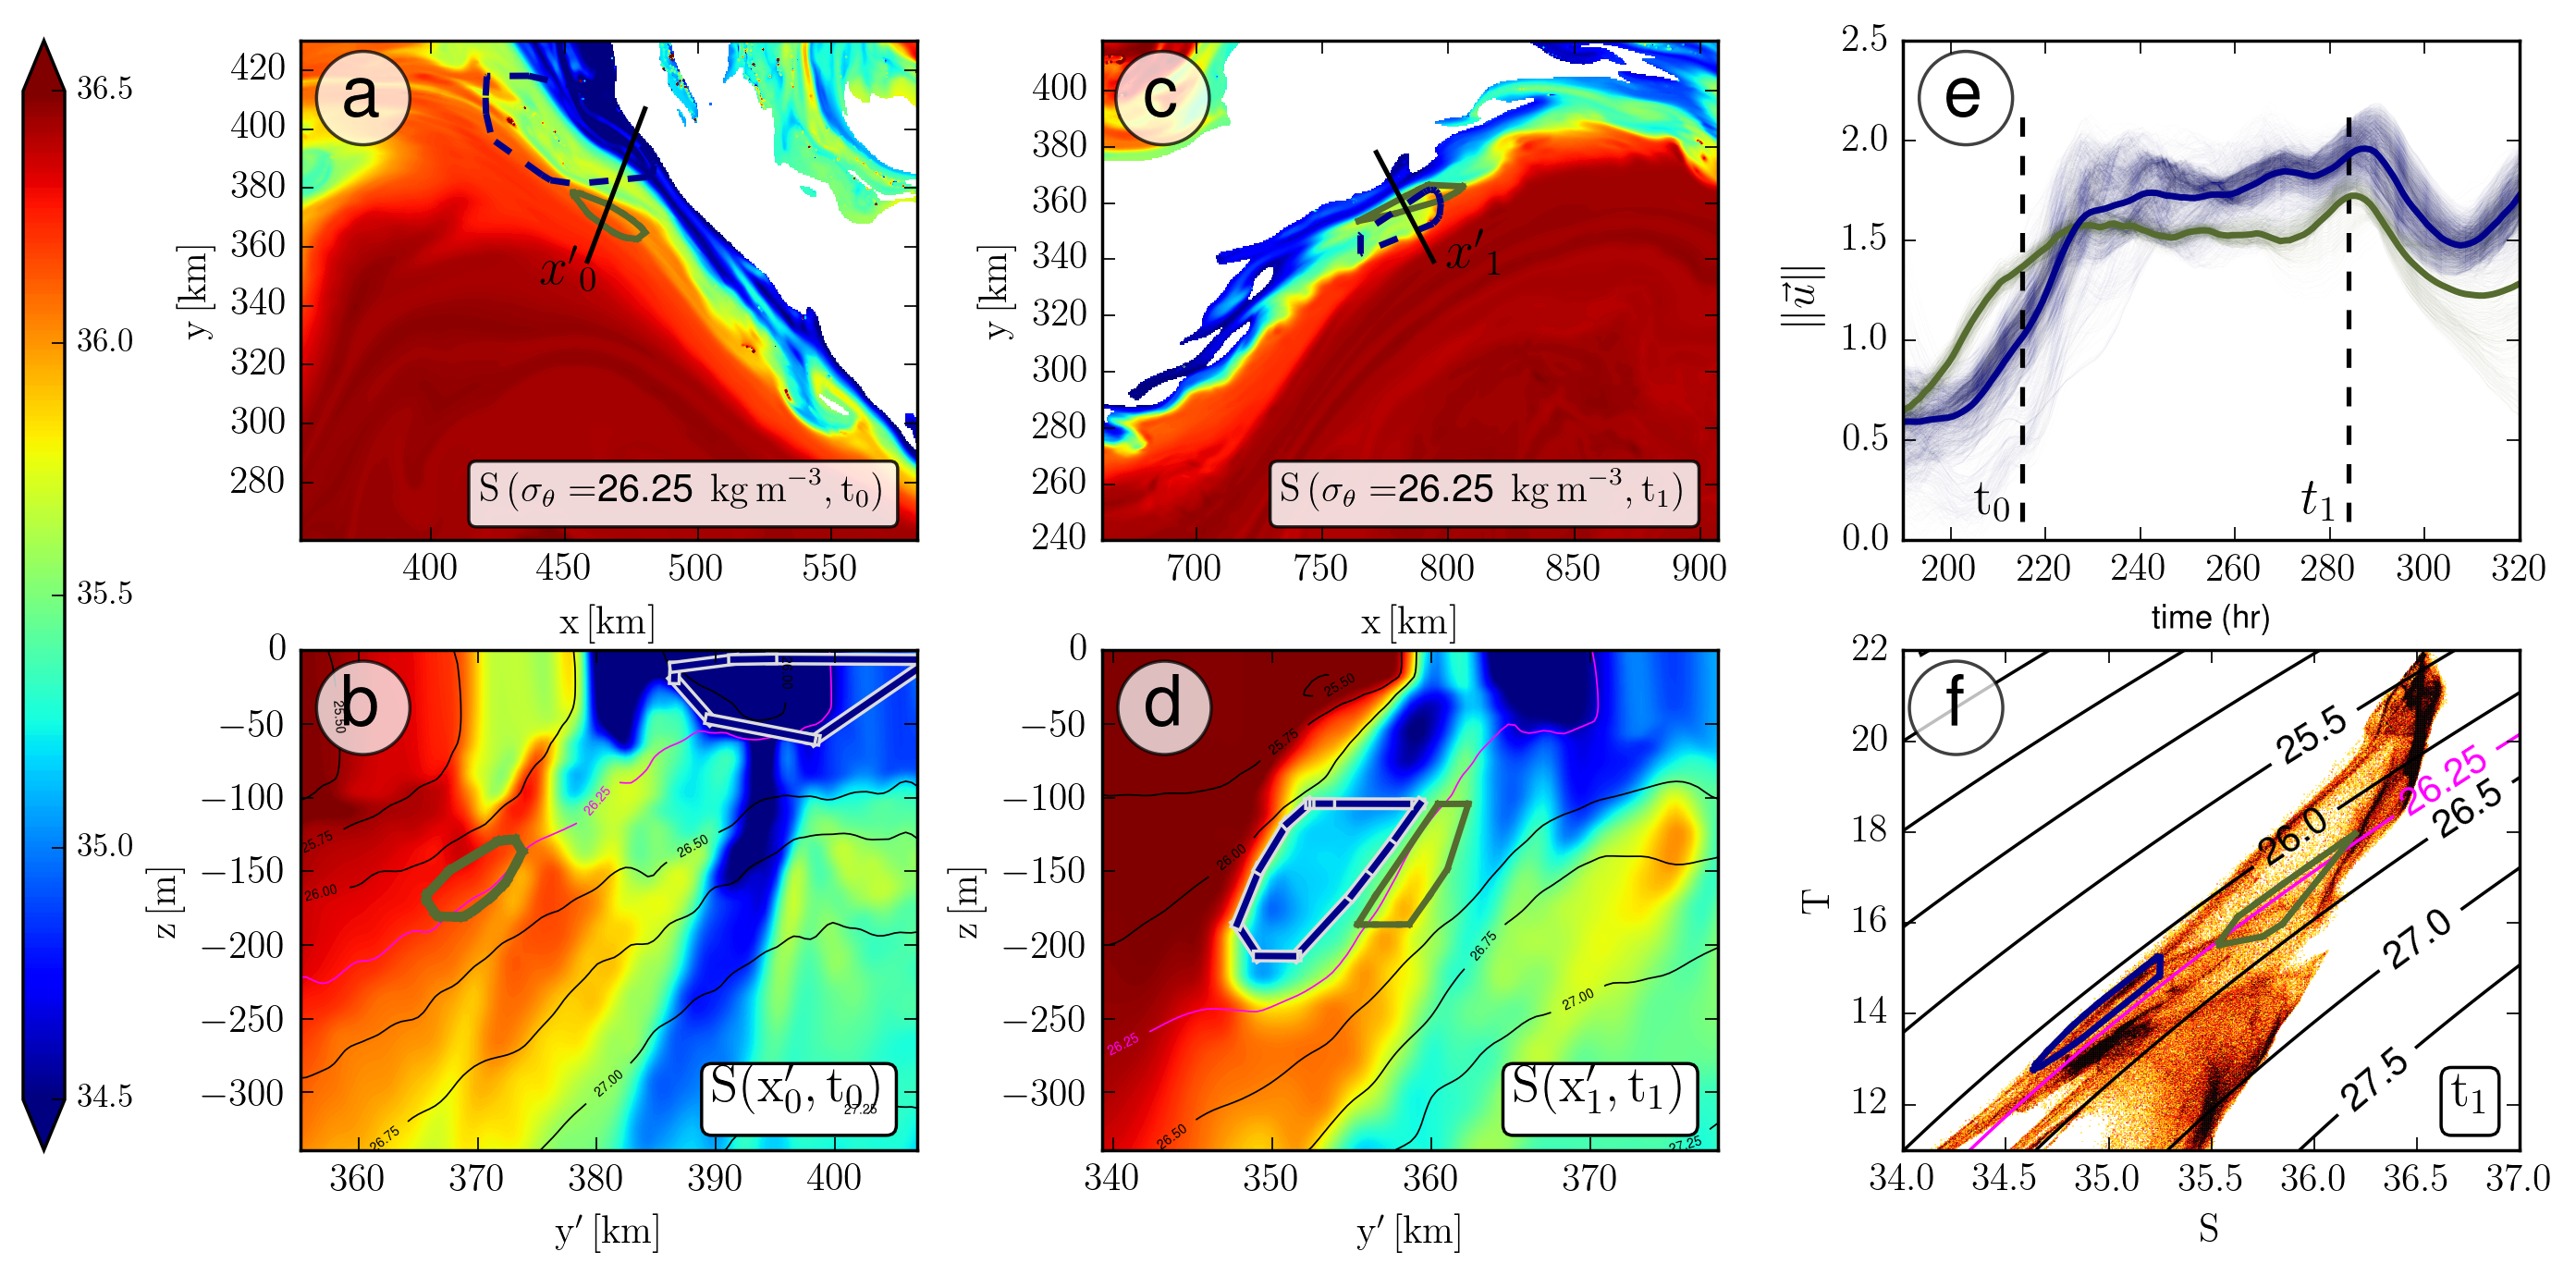
\includegraphics[width=0.9\textwidth]{./StreamersModel.png}
  \caption{{\bf Streamers and particles in a high-resolution simulation.}
a) Salinity in Gulf Stream on the $\sigma_{\theta}=26.25\  \mathrm{kg\,m^{-3}}$ isopycnal from a high-resolution numerical simulation at $t_0=215 \mathrm{h}$.  The green contours delineates the location of particles seeded downstream in the streamer at time $t_1=285 h$ (see panels c and d) and advected \emph{backwards} in time to $t_0$ showing where the streamer water originated. The blue contour is the location of particles seeded in the fresh intrusion.  The straight line shows the location of the salinity cross-section in the next panel.  b) Salinity cross section with isopycnals in black, the $\sigma_{\theta}=26.25\  \mathrm{kg\,m^{-3}}$ isopycnal in magenta, and the location of the particle cloud outlined in blue and green.  c) and d) are the same as a) and b) except for $t_1=285 \mathrm{h}$; the  cloud of particles outlined in green has been seeded in the streamer at this time, and the blue cloud has been seeded in the fresh intrusion.  e) The absolute speed of the particles (thin lines) and the average speed of the particles (thick lines) for the clouds contoured in a)--d).  Note that the green cloud has slowed relative to the blue cloud, indicating that the streamers have decelerated and the fresh intrusion has accelerated.  f) The temperature-salinity of all the data at $t_1$, with the clouds of seeded particles indicated in T/S space.  Note that the green ``streamer'' water occupies a partially mixed mode between the warm Gulf Stream waters and the cold and fresh water to the north.  
  } \label{fig:StreamersModel}
\end{figure*}


%% Put the bibliography here, most people will use BiBTeX in
%% which case the environment below should be replaced with
%% the \bibliography{} command.

\bibliography{main}

%\begin{thebibliography}{1}
%\bibitem{dummy} Articles are restricted to 50 references, Letters
%to 30.
%\bibitem{dummyb} No compound references -- only one source per
%reference.
%\end{thebibliography}


%% Here is the endmatter stuff: Supplementary Info, etc.
%% Use \item's to separate, default label is "Acknowledgements"

\begin{addendum}
 \item  Our thanks to the captains and crews of \emph{R/V Knorr} and \emph{R/V Atlantis}, The AVHRR Oceans Pathfinder SST data were obtained from the Physical Oceanography Distributed Active Archive Center (PO.DAAC) at the NASA Jet Propulsion Laboratory, Pasadena, CA. http://podaac.jpl.nasa.gov. Funding was supplied by Office of Naval Research, Grants XXXXXX
 \item[Competing Interests] The authors declare that they have no
competing financial interests.
 \item[Correspondence] Correspondence and requests for materials
should be addressed to Jody M. Klymak.~(email: jklymak@uvic.ca).
\end{addendum}

%%
%% TABLES
%%
%% If there are any tables, put them here.
%%

\end{document}
